\section{Simulation of Controller}

For the simulation the controller was implemented in Simulink, and it operates alongside the autopilot described in chapter \ref{ch:simulation}. Since the controller will be used to control course using the rudder, the autopilot will be controlling all the other states and actuators.


\subsection{Controller Implementation}

The controller was implemented using a simple block diagram in Simulink, with desired course as input and rudder control as output. As a starting point for the controller tuning the control loop was simulated in an open loop. 

\subsection{Test Cases}


The altitude used when using a pushbroom sensor from an UAV for ground observation varies with what is being observed and the equipment used. When observing the vegetation, low-altitudes around $100$ m is often used (\cite{hymsySUOMALAINEN}, \cite{wheatLELONG}, \cite{lowRAMIREZ}). However, altitudes as high as $1900$ m has been used to observe agricultural crops \cite{mosaicASMAT}. In this paper simulations will be performed mostly at $100$ m, with some simulations at higher altitudes for comparison. The FOV for the camera will be set to $19\degree$ (approximately the same as in \cite{hymsySUOMALAINEN}).

The controller has been tested in three different cases. The first case is a simple $45\degree$ turn in order to test the step response of the controller. The second case will follow a path in order to compare the controller with a "regular" course controller. The third and last case is the same path as in the second case, but with wind.


\subsection{Results: Step Response}

The step response of the controller is shown in figure \ref{fig:ratc_step_course}, together with the step response of a controller using the aileron to turn. The course angle $\chi$ reaches the desired $45\degree$ ($0.76$ $rad$) after about $80$ seconds. This is $20$ seconds after the aileron-controller starts to stabilize at $45\degree$, and while the aileron-controller is underdamped the rudder-controller is overdamped. Just after the step response has occured, the course angle for the rudder-controller starts off in the slightly wrong direction before it starts increasing.

\begin{figure}[]
    \centering
    \makebox[\textwidth][c]{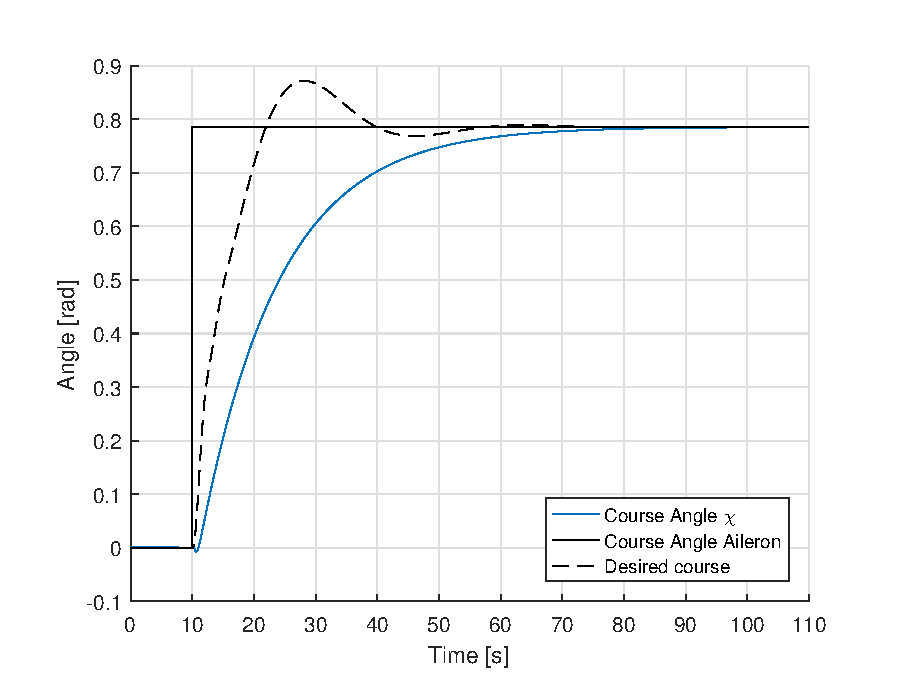
\includegraphics[width=1.2\textwidth, keepaspectratio=true]{../../results/controller/step/step_course.eps}}
    \caption{The step response of the course controller, compared to the course step response of a course controller using the ailerons.}
	\label{fig:ratc_step_course}
\end{figure}

\begin{figure}[]
    \centering
    \makebox[\textwidth][c]{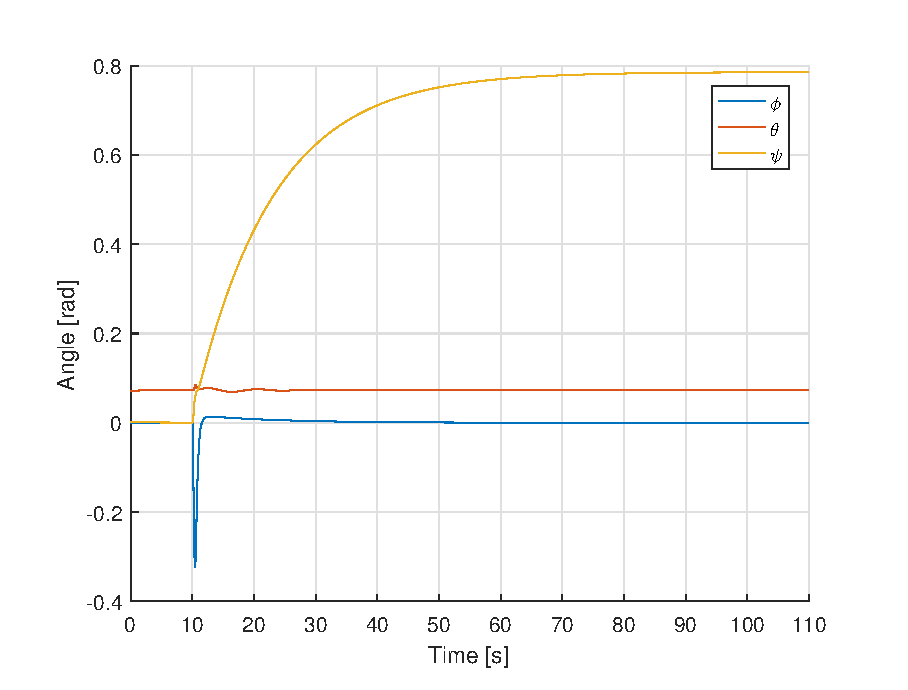
\includegraphics[width=1.2\textwidth, keepaspectratio=true]{../../results/controller/step/step_states.eps}}
    \caption{The attitude states of the UAV during the step response.}
	\label{fig:ratc_step_states}
\end{figure}

Figure \ref{fig:ratc_step_states} show that the pitch $\theta$ has only small variations when the step response occurs. When the step occurs the roll $\psi$ changes rapidly back and forth. This is because the deflection of the rudder actuator also induces a roll on the aircraft. This can also be seen on the inputs shown in figure \ref{fig:ratc_step_input}. At the time of the step both the aileron and the rudder increases rapidly, with an almost "mirrored" response.

\begin{figure}[]
    \centering
    \makebox[\textwidth][c]{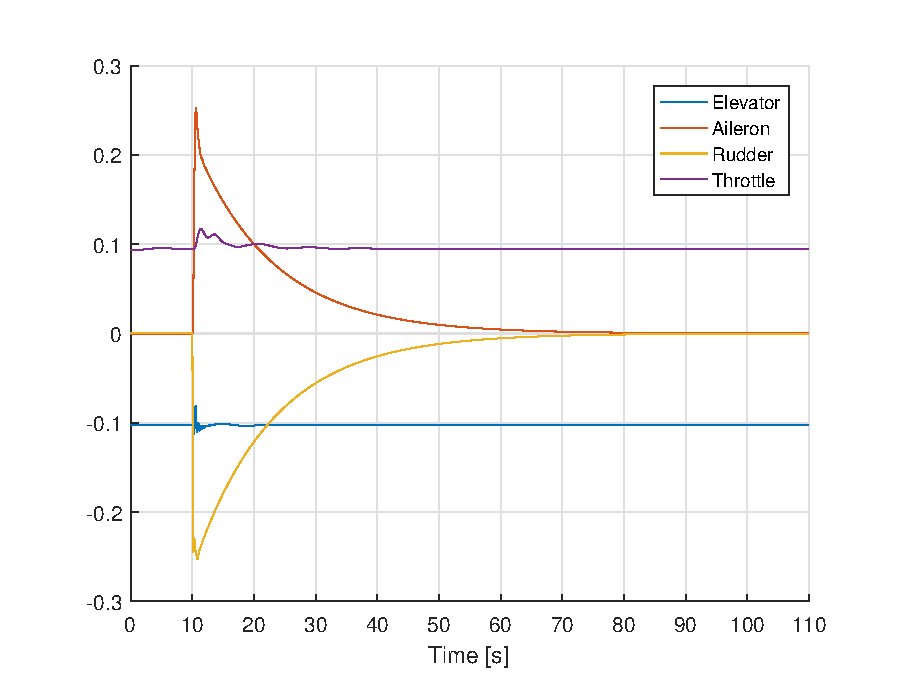
\includegraphics[width=1.2\textwidth, keepaspectratio=true]{../../results/controller/step/step_input.eps}}
    \caption{Input used during the step response. The input is given as a signal between $\pm1$.}
	\label{fig:ratc_step_input}
\end{figure}

The bode-plot in figure \ref{fig:ratc_bode} shows the frequency response of the rudder controller. The phase margin is $61.2\degree$ and since the pase never goes below $-180\degree$, this is a stable system (REFERERE TIL ANDRESEN). This tuning was achieved with $\zeta$ set to $42$ and $\omega_n$ set to $42$, which corresponds to a $k_p$ of $42$ and a $k_d$ of $42$.

\begin{figure}[]
    \centering
    \makebox[\textwidth][c]{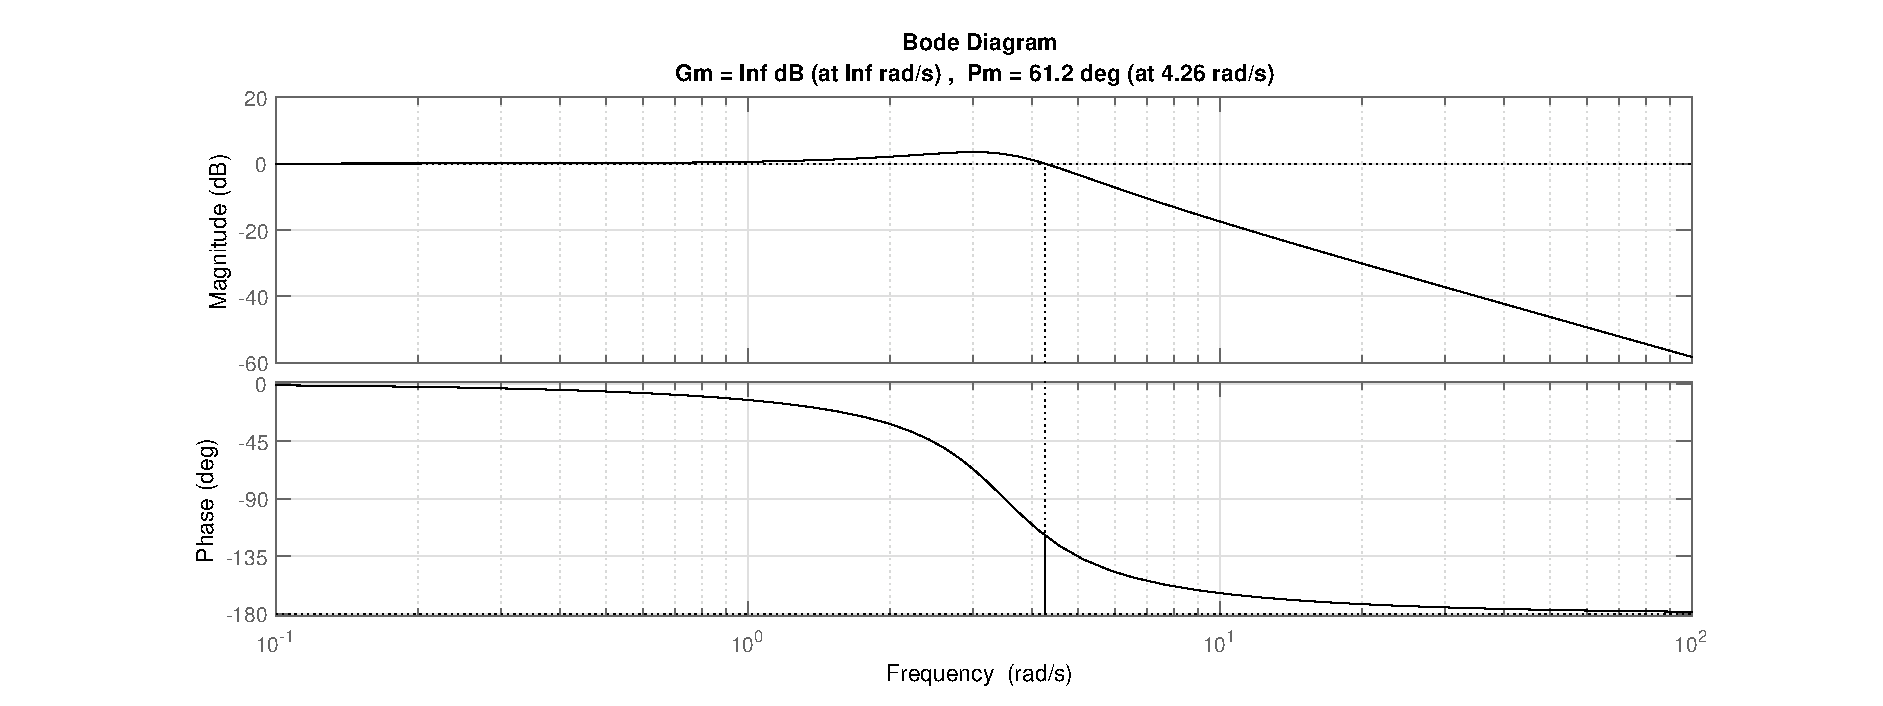
\includegraphics[width=1.2\textwidth, keepaspectratio=true]{../../results/controller/step/bode.eps}}
    \caption{The camera footprint during simulation of the first path.}
	\label{fig:ratc_bode}
\end{figure}


\subsection{Results: Path}

The results of the simulation for the rudder controller can be seen in figures \ref{fig:ratc_path_hundred} and \ref{fig:ratc_comp_hundred}. The figures show that the controller manages to keep the ground path that is to be observed within the camera footprint when the path is straight. However, it does need to be a sharp turn for the camera to shift away from the ground path. The effect of the roll that the rudder induces, which can be seen in figure \ref{fig:ratc_step_states} with the step response, is also visible on the camera footprint. At the beginning of each turn there are a small "NUDGE" in the footprint, but none of them moves the camera outside the observation path.

\begin{figure}[]
    \centering
    \makebox[\textwidth][c]{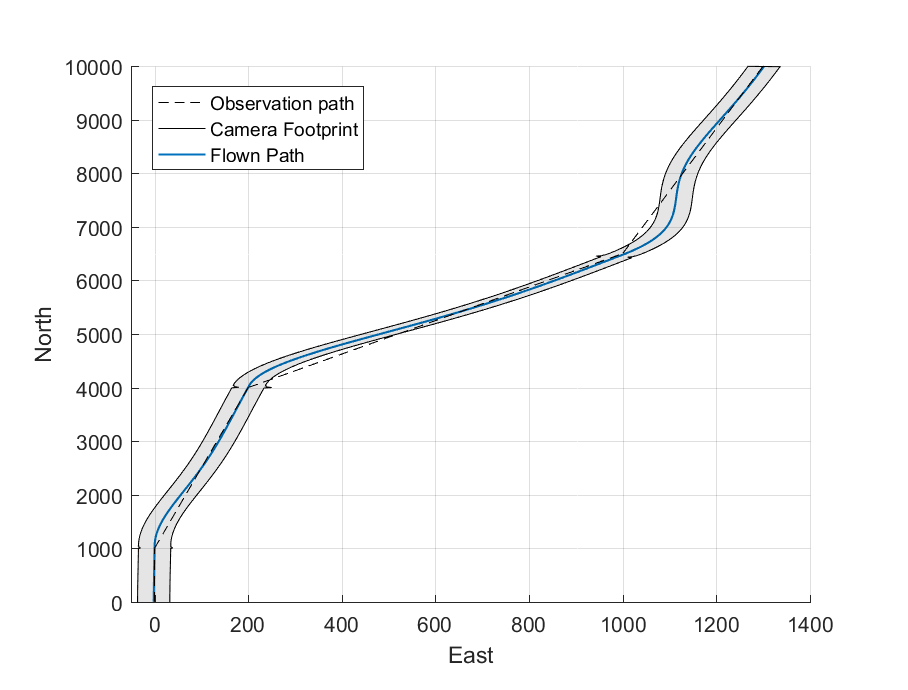
\includegraphics[width=1.2\textwidth, keepaspectratio=true]{../../results/controller/path/ratc_path_hundred.eps}}
    \caption{The path flown and the camera footprint when following the path using the rudder controller. Altitude is $100$ m.}
	\label{fig:ratc_path_hundred}
\end{figure}

\begin{figure}[]
    \centering
    \makebox[\textwidth][c]{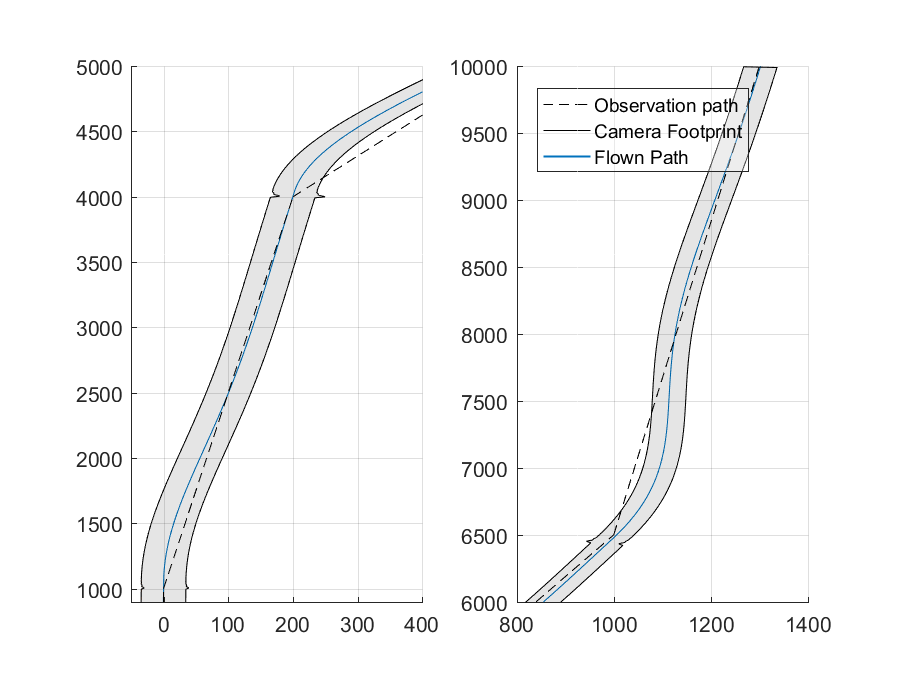
\includegraphics[width=1.2\textwidth, keepaspectratio=true]{../../results/controller/path/ratc_comp_hundred.eps}}
    \caption{Detailed view of the path flown and the camera footprint when following the path using the rudder controller. Altitude is $100$ m.}
	\label{fig:ratc_comp_hundred}
\end{figure}

The flown path and the camera footprint for the controller using the aileron to change course is shown in figures \ref{fig:aotc_path_hundred} and \ref{fig:aotc_comp_hundred}. The obsevation path is within the camera footprint almost throughout the flight, but the edge of the camera footprint is close to the observation path at multiple times. At the beginning of every turn there is rapid shift in the camera footprint because of an abrupt roll change, and after every turn the roll of the aircraft is swining back and forth before it settles.

\begin{figure}[]
    \centering
    \makebox[\textwidth][c]{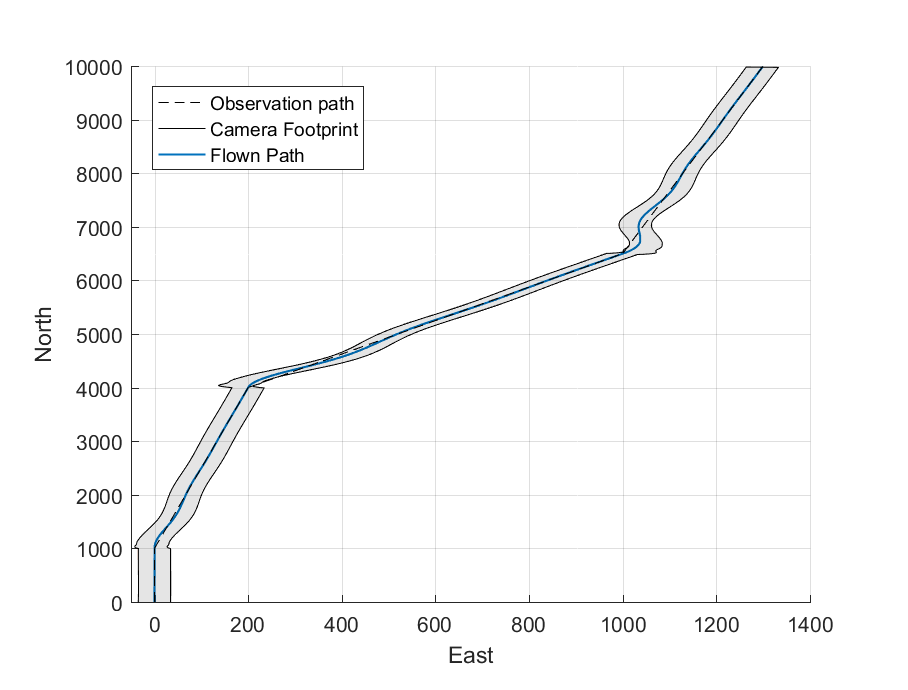
\includegraphics[width=1.2\textwidth, keepaspectratio=true]{../../results/controller/path/aotc_path_hundred.eps}}
    \caption{The path flown and the camera footprint when following the path using the aileron controller. Altitude is $100$ m.}
	\label{fig:aotc_path_hundred}
\end{figure}

\begin{figure}[]
    \centering
    \makebox[\textwidth][c]{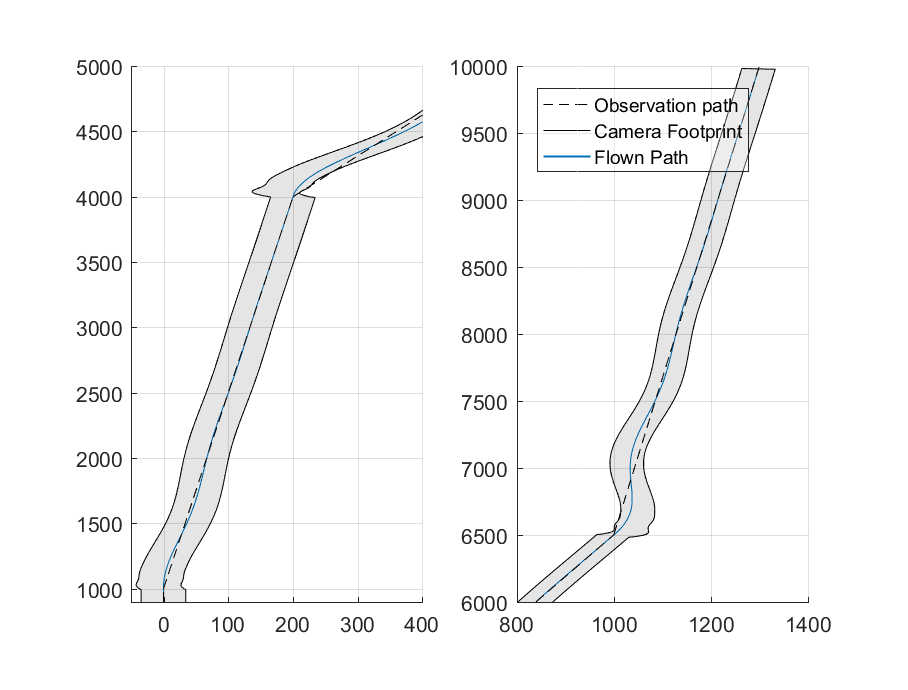
\includegraphics[width=1.2\textwidth, keepaspectratio=true]{../../results/controller/path/aotc_comp_hundred.eps}}
    \caption{Detailed view of the path flown and the camera footprint when following the path using the aileron controller. Altitude is $100$ m.}
	\label{fig:aotc_comp_hundred}
\end{figure}

The camera footprint for the two paths are shown in figure \ref{fig:ratc_aotc_comparison}. The figure shows that the camera footprint of the aileron controller SWINGS more than the footprint of the rudder controller, but it doesn't necessarily move further away from the observaton path. At the beginning of the turns both of the controllers causes a "NUDGE" in the camera footprint in opposite directions. The "NUDGE" of the aileron controller is bigger and remains longer than the "NUDGE" for the rudder controller.

\begin{figure}[]
    \centering
    \makebox[\textwidth][c]{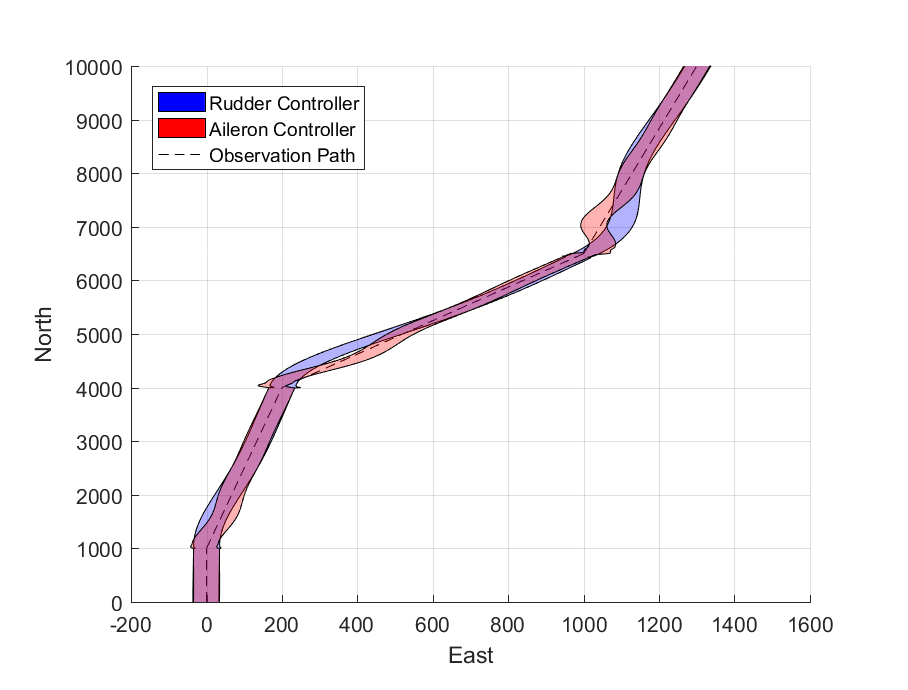
\includegraphics[width=1.2\textwidth, keepaspectratio=true]{../../results/controller/path/comparison.eps}}
    \caption{A comparison of the camera footprints of the two controllers. Altitude is $100$ m.}
	\label{fig:ratc_aotc_comparison}
\end{figure}